\documentclass[border=1pt]{standalone}
\usepackage{tikz}
\usepackage{luatexja}
\usetikzlibrary{decorations.markings}

\begin{document}
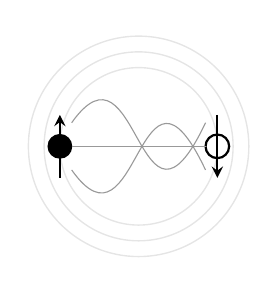
\begin{tikzpicture}
    % 背景の円環（量子的なゆらぎ）
    \foreach \r in {1, 1.2, 1.4} {
        \draw[black!10, line width=0.5pt] (0,0) circle (\r);
    }
    % 粒子（スピンの対比）
    \draw[fill=black] (-1,0) circle (0.15);
    \draw[fill=white, thick] (1,0) circle (0.15);
    
    % スピンベクトル
    \draw[-stealth, thick] (-1, -0.4) -- (-1, 0.4);
    \draw[-stealth, thick] (1, 0.4) -- (1, -0.4);
    
    % もつれを象徴する曲線
    \foreach \s in {-0.3, 0, 0.3} {
        \draw[black!40, thin] (-0.85, \s) .. controls (0, \s*5) and (0, -\s*5) .. (0.85, \s);
    }
\end{tikzpicture}
\end{document}
